\chapter{Implementacja sterowania NAO}
\section{Interfejs robota NAO}

Aby zasymulować robota skorzystano z trzech narzędzi. 

Wymagana jest wersja 2.1.2 NAOqi i Choreographe, ponieważ kolejnie nie są ze sobą w pełni kompatybilne z ROSem.

\subsubsection{NAOqi} System operacyjny oparty o jądro Linux autorstwa firmy Aldebaran, pozwalający na sterowanie robotem NAO, programowanie go oraz utworzenie wirtualnego agenta podłączonego do symulacji. Instancja NAOqi działa na komputerze pokładowym robota. Producent dostarcza zestaw narzędzi, pozwalających na pisanie programów w językach C++, Java lub Python. NAOqi może zostać uruchomione niezależnie od innych aplikacji z poziomu terminala.

\subsubsection{Choreographe} Aplikacja okienkowa, umożliwiająca tworzenie scenariuszy działania robota w formie graficznej. Choreographe dostarcza bibliotekę akcji w postaci bloków, możliwych do połączenia przez programistę w automat skończony. Dzięki aplikacji można w łatwy sposób podłączyć się do fizycznego robota, utworzyć symulację, bądź połączyć się z działającą w systemie insntacją NAOqi. W jednej z zakładek można zobaczyć wizualizację stanu robota, która działa wydajniej, niż inne dostępne rozwiązania.

\subsubsection{ROS} Oprogramowanie ułatwiające sterowanie robotami. Zapewnia zbiór narzędzi umożliwiających nadawanie i odbieranie wiadomości, tworzenie symulacji, szkielet architektury wiadomości i serwisów, zewnętrzne biblioteki, integracja z Pythonem, C++, przeglądarkami internetowymi.

Oprogramowanie ułożone w pakiety, ROS potrafi sam zadbać o odpowiednie zależności.

Integracja z ROSem może otworzyć dodatkowe możliwości, takie jak komunikacja z otoczeniem i innymi robotami, poszerzenie zmysłów, poprzez integrację zewnętrznych czujników. 
\\\\
Po zaimportowaniu biblioteki \textit{rospy} oraz klasy \textit{ALProxy} z biblioteki \textit{naoqi} możliwe było połączenie się z robotem. Wymagało to użycia trzech linijek kodu: definiującej numery IP, numer portu oraz aktywującej  Przy korzystaniu z symulacji należy podmienić numer portu

\ktem. W tym celu zdefiniowano klasę \textit{Robot}, której konstuktor laALProxy z broboiblioteki NAOqi.sy lliwe Możstinputlisting[language=Python,linerange=7-11,firstnumber=7]{scripts/robot.py}
\lstinputlisting[language=Python,linerange=14-17,firstnumber=14]{scripts/robot.py}


\section{SMACH}

\subsection{Koncepcja zastosowania}
Robot Nao nie posiada wbudowanego automatu skończonego. Dlatego celowe wydaje się zintegrowanie jego działania z zewnętrznym narzędziem do tworzenia automatów. 
Zadanie można zrealizowac z użyciem SMACH (skrót od "State Machine"). Biblioteka ta została stworzona przez deweloperów ROSa, ale jest od niego niezależna i może być używana osobno. 

\subsection{Implementacja}
Pakiet SMACH jest instalowany domyślnie z ROSem. Z poziomu Pythona biblioteka jest importowana bez żadnych dodatkowych działań.

\subsection{Weryfikacja koncepcji}
SMACH pozwala na tworzenie wysokopoziomowej warstwy sterowania robotem. Możliwe jest tworzenie prostych scenariuszy w postaci maszyn stanu. Dzięki modułowości architektury SMACHa, można wykorzystać je jako elementy większych sceraniuszy. 

Dzięki integracji z ROSem SMACH udostępnia interfejs do analizy stanu automatu w czasie rzeczywistym. 

Działanie automatu skończonego ciężko nazwać inteligentnym. Robot nie planuje samodzielnie zadań. Programista jest zmuszony do przewidzenia wszystkich możliwych scenariuszy działania. 

SMACH wymaga zdefiniowania wszystkich możliwych stanów i zasad przejścia między stanami przed rozpoczęciem swojego działania. Jego działanie ma charakter statyczny i nie może być dostosowywane w trakcie realizacji programu. Wymaga to od programisty mądrego przemyślenia architektury systemu i uwzględnienia ewentualnych problemów przy realizacji zadania (np. kolizji robota z przeszkodą). 

% Mimo to, właśnie automaty skończone są podstawową metodą wykorzystywaną do interakcji robot - człowiek.

\begin{figure}
\centering
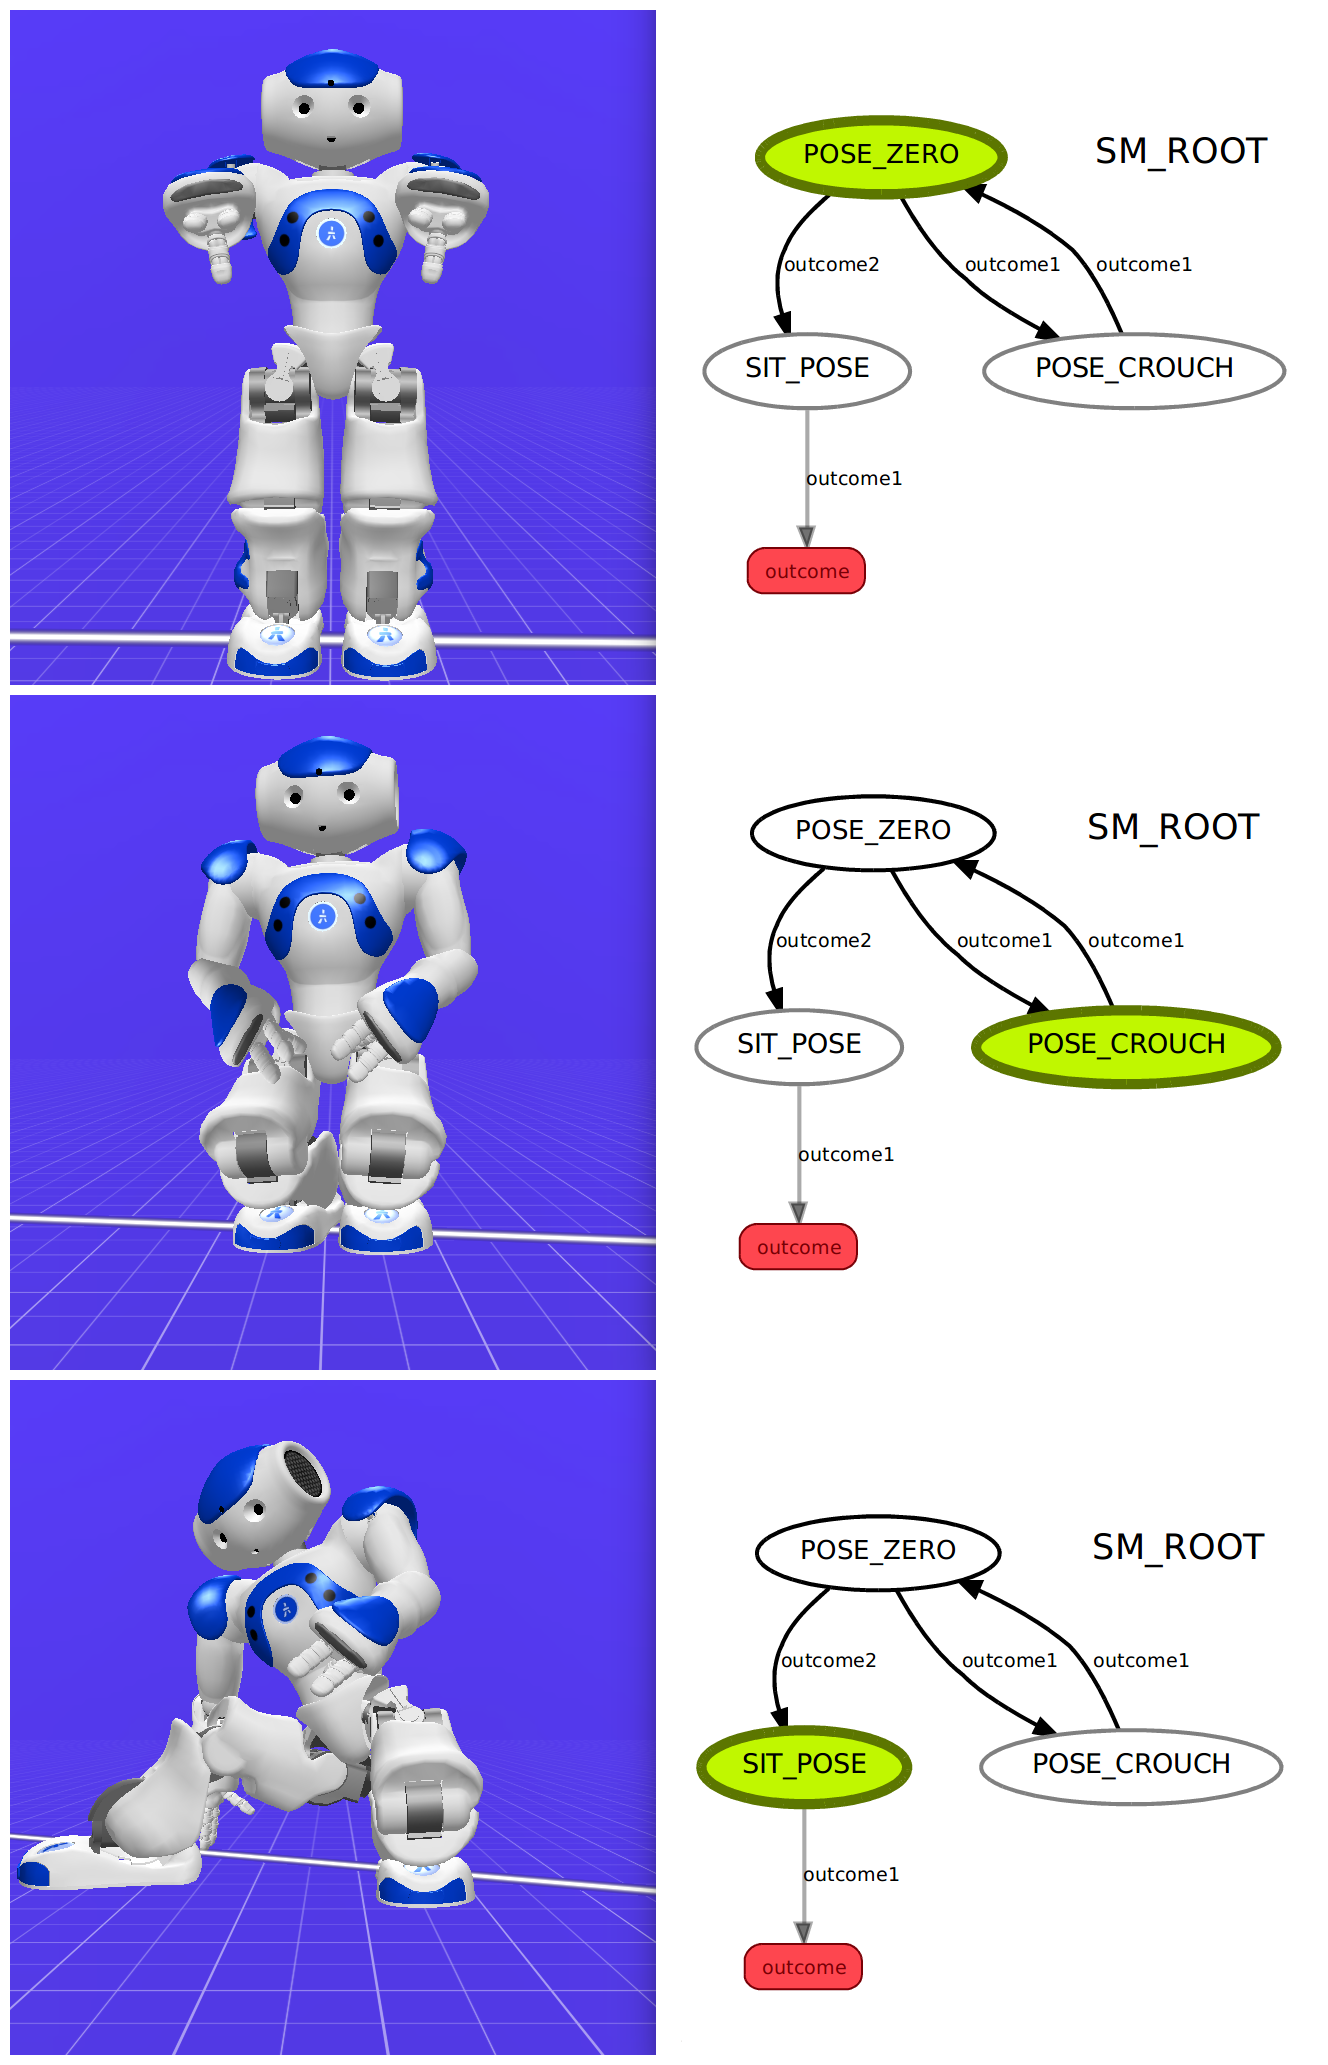
\includegraphics[width=0.90\textwidth]{images/NaoSmachPoses.png}
\caption{Wirtualny robot zwizualizowany w Choreographe sterowany przez automat stanu SMACH.}
\end{figure}


\section{RGOAP}

\subsection{Koncepcja zastosowania}
Maszyny stanu pozwalają na realizację przez robota scenariuszów, jednak każdy z nich musi być zaplanowany osobno. Wymaga to dużego nakładu pracy, więc zasadnym jest podjęcie próby automatyzacji tego procesu. GOAP na podstawie warunków i efektów zdefiniowanych wcześniej akcji pozwala na automatyczne łączenie ich w proste lub bardziej skomplikowane scenariusze. 

\subsection{Implementacja}
RGOAP powstało w 2013 roku, jako pakiet ROSa w wersji Groovy. Do budowy pakietu należy wykorzystać narzędzie rosbuild. Jest to problematyczne, ponieważ aktualnie wspieranym narzędziem tworzenia i budowy pakietów jest Catkin. Z tego powodu w trakcie realizacji pracy przebudowano strukturę plików pakietu, catkinizując RGOAP. Efekt pracy można pobrać z repozytorium autora: \url{https://github.com/juliusz-t/executive_rgoap/tree/catkin}

\subsection{Weryfikacja koncepcji}

Projektowanie scenariuszy w FSM i GOAP może mieć bardzo podobny efekt. Jednak w FSM naturalniejszym rozwiązaniem wydaje się okreslenie wierzchołków grafu jako statycznych stanów i krawędzi grafu, jako dynamicznych akcji. GOAP będąc bardziej intuicyjny zmusza do okreslania wierzchołków grafu jako akcji, a krawędzi jako momentów w których stan świata jest czasowo statyczny. Uzyskane w ten sposób grafy mogą być dualne względem siebie.

\subsection{Możliwość zastosowania w poznawczych modelach umysłu}

% \section{Porównanie SMACH i RGOAP}
% FSM jako statyczny, GOAP jako dynamiczny system podejmowania decyzji.
